\documentclass[12pt,a4paper]{article}

\usepackage{graphicx}
\usepackage[a4paper,margin=0.8in]{geometry}
\usepackage{changepage}
\usepackage{float}
\usepackage{url}
\usepackage{amsmath}
\usepackage{tabularx}
\usepackage{titlesec}
\usepackage{listings}
\usepackage{xcolor}
\usepackage{tikz}
\usetikzlibrary{automata, positioning, arrows, shapes.geometric}

\definecolor{codegreen}{rgb}{0,0.6,0}
\definecolor{codegray}{rgb}{0.5,0.5,0.5}
\definecolor{codepurple}{rgb}{0.58,0,0.82}
\definecolor{backcolour}{rgb}{0.95,0.95,0.92}

\lstdefinestyle{mystyle}{
    backgroundcolor=\color{backcolour},   
    commentstyle=\color{codegreen},
    keywordstyle=\color{magenta},
    numberstyle=\tiny\color{codegray},
    stringstyle=\color{codepurple},
    basicstyle=\ttfamily\footnotesize,
    breakatwhitespace=false,         
    breaklines=true,                 
    captionpos=b,                    
    keepspaces=true,                 
    numbers=left,                    
    numbersep=5pt,                  
    showspaces=false,                
    showstringspaces=false,
    showtabs=false,                  
    tabsize=4
}
\lstset{style=mystyle}

\titleformat{\section}
  {\bfseries}
  {\thesection.}{0.5em}{}

\titleformat{\subsection}
  {\large\bfseries}
  {\thesubsection}{1em}{}


\title{Computer Architecture Lab 06}
\author{Group 15}
\date{\today}

\begin{document}

\begin{center}
{\Large \textbf{Department of Computer Engineering}}\\
\vspace{0.2cm}
{\large University of Peradeniya}\\
\vspace{0.6cm}

{\large CO2070 -- COMPUTER ARCHITECTURE}\\
\vspace{0.3cm}
{\Large \textbf{LAB 06 REPORT}}\\
\vspace{0.2cm}

\end{center}
{\large
\textbf{Team Number:} No. 15\\[0.3cm]
\textbf{Name:} K.D.N.Chandrasena\\[0.3cm]
\textbf{Registration Number:} E/22/054\\[0.3cm]
\textbf{Date:} \today
}

\vspace{1cm}

% ============================================================
% SECTION 1
% ============================================================
\section*{1. Handling Cache Misses}

\textbf{Memory Write Policies:}
\begin{itemize}
    \item \textbf{Write-Through:} Cache and Main Memory are updated simultaneously. Slower due to memory delays on every write.
    \item \textbf{Write-Back (Used):} Only Cache is updated. A \textbf{Dirty Bit} marks modified blocks. Main memory is only updated when a dirty block is evicted.
\end{itemize}

\textbf{Miss Handling (Write-Back):}
\begin{enumerate}
    \item \textbf{Stall:} CPU is stalled (\texttt{BUSYWAIT = 1}).
    \item \textbf{Evict (if necessary):} If the current block is Dirty, write it back to Main Memory.
    \item \textbf{Fetch:} Read the new block from Main Memory.
    \item \textbf{Update:} Set Tag, \texttt{Valid = 1}, and \texttt{Dirty = 0}.
    \item \textbf{Execute:} 
        \begin{itemize}
            \item \textit{Read Miss:} Return requested byte.
            \item \textit{Write Miss:} Write new data into cache block, set \texttt{Dirty = 1}.
        \end{itemize}
    \item \textbf{Resume:} CPU unstalled (\texttt{BUSYWAIT = 0}).
\end{enumerate}

\begin{figure}[H]
\centering
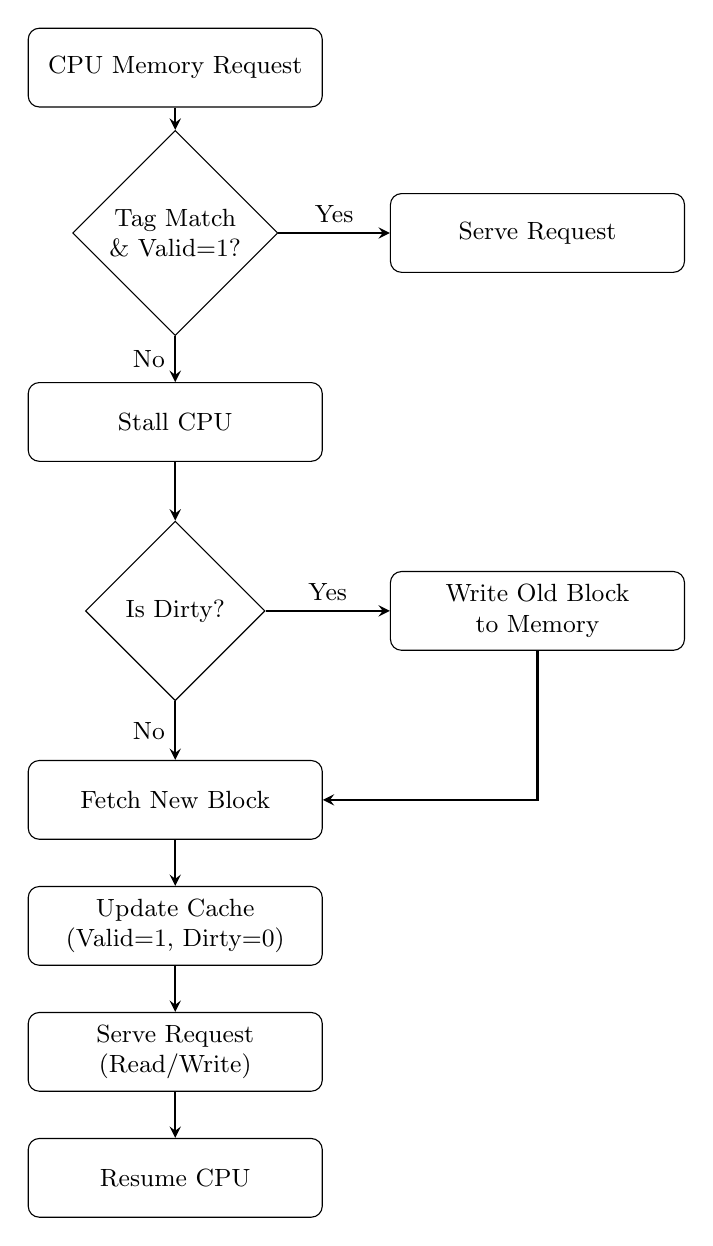
\begin{tikzpicture}[node distance=1.6cm,
  process/.style={rectangle, draw, rounded corners, text width=3.5cm, text centered, minimum height=1cm, font=\small},
  decision/.style={diamond, draw, text width=2cm, text centered, inner sep=0pt, font=\small},
  arrow/.style={thick,->,>=stealth}]
  
  \node (start) [process] {CPU Memory Request};
  \node (checkhit) [decision, below of=start, yshift=-0.5cm] {Tag Match \& Valid=1?};
  \node (hit) [process, right of=checkhit, xshift=3cm] {Serve Request};
  \node (stall) [process, below of=checkhit, yshift=-0.8cm] {Stall CPU};
  \node (checkdirty) [decision, below of=stall, yshift=-0.8cm] {Is Dirty?};
  \node (writeback) [process, right of=checkdirty, xshift=3cm] {Write Old Block to Memory};
  \node (fetch) [process, below of=checkdirty, yshift=-0.8cm] {Fetch New Block};
  \node (update) [process, below of=fetch] {Update Cache (Valid=1, Dirty=0)};
  \node (resolve) [process, below of=update] {Serve Request (Read/Write)};
  \node (resume) [process, below of=resolve] {Resume CPU};

  \draw [arrow] (start) -- (checkhit);
  \draw [arrow] (checkhit) -- node[anchor=south, font=\small] {Yes} (hit);
  \draw [arrow] (checkhit) -- node[anchor=east, font=\small] {No} (stall);
  \draw [arrow] (stall) -- (checkdirty);
  \draw [arrow] (checkdirty) -- node[anchor=south, font=\small] {Yes} (writeback);
  \draw [arrow] (writeback) |- (fetch);
  \draw [arrow] (checkdirty) -- node[anchor=east, font=\small] {No} (fetch);
  \draw [arrow] (fetch) -- (update);
  \draw [arrow] (update) -- (resolve);
  \draw [arrow] (resolve) -- (resume);
\end{tikzpicture}
\end{figure}

\newpage

% ============================================================
% SECTION 2
% ============================================================
\section*{2. Cache Mapping Mechanism}

\textbf{Mechanism:} Direct Mapped Cache\\
\textbf{Address Size:} 8 bits

\begin{itemize}
    \item \textbf{Offset:} 4 Bytes per block $\rightarrow$ 2 bits.
    \item \textbf{Index:} 8 lines in cache $\rightarrow$ 3 bits.
    \item \textbf{Tag:} Remaining bits $\rightarrow$ 3 bits.
\end{itemize}

\begin{table}[H]
\centering
\begin{tabular}{|c|c|c|}
\hline
\textbf{Tag (3 bits)} & \textbf{Index (3 bits)} & \textbf{Offset (2 bits)} \\ \hline
Bits [7:5] & Bits [4:2] & Bits [1:0] \\ \hline
\end{tabular}
\end{table}

% ============================================================
% SECTION 3
% ============================================================
\section*{3. Cache Table Trace}

\begin{itemize}
    \item \texttt{loadi 0 0x09} $\rightarrow$ R0 = \texttt{0x09}. (No cache operation)
    \item \texttt{loadi 1 0x01} $\rightarrow$ R1 = \texttt{0x01}. (No cache operation)
    \item \texttt{swd 0 1} $\rightarrow$ Mem[0x01] = 0x09 (Index 0). Write Miss. Fetches Block 0, writes 0x09 to Offset 1. (Dirty = 1)
    \item \texttt{swi 1 0x00} $\rightarrow$ Mem[0x00] = 0x01 (Index 0). Write Hit. Writes 0x01 to Offset 0. (Dirty = 1)
    \item \texttt{lwd 2 1} $\rightarrow$ R2 = Mem[0x01]. Read Hit (Index 0).
    \item \texttt{lwd 3 1} $\rightarrow$ R3 = Mem[0x01]. Read Hit (Index 0).
    \item \texttt{sub 4 0 1} $\rightarrow$ R4 = R0 - R1 = 0x08. (No cache operation)
    \item \texttt{swi 4 0x07} $\rightarrow$ Mem[0x07] = 0x08 (Index 1). Write Miss. Fetches Block 1, writes 0x08 to Offset 3. (Dirty = 1)
    \item \texttt{lwi 5 0x07} $\rightarrow$ R5 = Mem[0x07]. Read Hit (Index 1).
    \item \texttt{lwi 6 0x20} $\rightarrow$ R6 = Mem[0x20] (Index 0, Tag 1). Read Miss. Evicts dirty Block 0. Fetches Block 8. (Dirty = 0)
    \item \texttt{swi 4 0x20} $\rightarrow$ Mem[0x20] = 0x08 (Index 0, Tag 1). Write Hit. Writes 0x08 to Offset 0. (Dirty = 1)
\end{itemize}

\begin{table}[H]
\centering
\renewcommand{\arraystretch}{1.2}
\begin{tabular}{|c|c|c|c|l|}
\hline
\textbf{Index} & \textbf{Valid} & \textbf{Dirty} & \textbf{Tag} & \textbf{Data (Bytes 0, 1, 2, 3)} \\ \hline
0 & 1 & 1 & 001 & \texttt{0x08}, XX, XX, XX \\ \hline
1 & 1 & 1 & 000 & XX, XX, XX, \texttt{0x08} \\ \hline
2 & 0 & 0 & 000 & XX, XX, XX, XX \\ \hline
3 & 0 & 0 & 000 & XX, XX, XX, XX \\ \hline
4 & 0 & 0 & 000 & XX, XX, XX, XX \\ \hline
5 & 0 & 0 & 000 & XX, XX, XX, XX \\ \hline
6 & 0 & 0 & 000 & XX, XX, XX, XX \\ \hline
7 & 0 & 0 & 000 & XX, XX, XX, XX \\ \hline
\end{tabular}
\end{table}

\newpage

% ============================================================
% SECTION 4
% ============================================================
\section*{4. Cache Controller FSM}

\begin{figure}[H]
\centering
\includegraphics[width=0.9\textwidth]{"Cache Controller FSM_complete.png"}
\end{figure}

\end{document}
